% !TeX program = xelatex
% Compile: xelatex sdd.tex && xelatex sdd.tex
\documentclass[12pt,a4paper]{article}
\usepackage{mondaiy-document-style}
\usepackage{graphicx}
\usepackage{pdflscape}
\graphicspath{{../gate-2/diagram/}}
\setlength{\LTpre}{6pt}
\setlength{\LTpost}{6pt}
\mondaiysetup{TÀI LIỆU THIẾT KẾ PHẦN MỀM}{SDD}{Software Design Document}
\begin{document}

\mondaiycover
  {TÀI LIỆU THIẾT KẾ PHẦN MỀM}
  {Software Design Document}
  {SDD}
  {IEEE 1016}
  {Thiết kế bám theo mã nguồn hiện có và artifact Gate 2}
\mondaiyfrontmatter

\section*{TÓM TẮT}
\addcontentsline{toc}{section}{TÓM TẮT}
\begin{keybox}[Vai trò tài liệu]
SDD này mô tả cách mondaiy đang được phân rã và vận hành trong repository:
client, FastAPI API, worker, connector, agent/tool, dữ liệu, UI/UX, security,
observability và deployment. Chỉ mô tả thành phần, contract và ràng buộc đã có
trong code/tài liệu kiến trúc liên quan; không đưa ra phương án thay thế.
\end{keybox}

\mondaiymetadata
  {MONDAIY-SDD-001}
  {Dũng --- PO/QC, design owner}
  {Dũng, Phong, An, Nhi}
  {Thiết kế thực thi SRS, truy vết tới code và STD.}

\section{Giới thiệu}
\subsection{Mục đích}
SDD xác định kiến trúc phần mềm, module, dữ liệu, giao tiếp giữa thành phần,
tích hợp bên ngoài, API, security, reliability, deployment và quyết định kỹ
thuật để hiện thực SRS. Mỗi mục trả lời module nào chịu trách nhiệm, input nào
được nhận, xử lý theo contract nào, output nào được tạo và failure nào phải
được báo ra. SDD không viết lại toàn bộ requirement của SRS.

\subsection{Phạm vi}
Phạm vi là các capability đã hiện diện trong repository: authentication,
connection/source sync, evidence và retrieval, conversation/agent/tool, task,
calendar, reminder, meeting notes, file intake, notification, mobile client,
browser extension, observability và deployment. SRS/PRD xác định yêu cầu sản
phẩm; migration và mã nguồn là nguồn chuẩn của trạng thái hiện thực.

\subsection{Định nghĩa và chữ viết tắt}
\begin{longtable}{p{3.0cm}p{11.5cm}}
\caption{Thuật ngữ thiết kế dùng xuyên suốt SDD}\label{tab:sdd-terms}\\
\toprule Thuật ngữ & Nghĩa \\ \midrule
\endfirsthead
\toprule Thuật ngữ & Nghĩa \\ \midrule
\endhead
AI & Artificial Intelligence; chỉ hỗ trợ hiểu, đề xuất và soạn draft. \\
LLM & Large Language Model; provider/model được backend chọn theo capability lane. \\
OAuth & Cơ chế ủy quyền để connector đọc nguồn theo quyền user cấp. \\
Evidence & Nội dung có source identity, provenance, timestamp và scope. \\
Context & Unified work context đã normalize, scope-filter và gắn evidence. \\
Action draft & Đề xuất task/calendar/reminder có thể sửa, chưa là external write. \\
Run & Một lần pipeline/agent thực thi có state, count, error class và correlation ID. \\
\bottomrule
\end{longtable}

\subsection{Nguồn tham chiếu bắt buộc}
\begin{longtable}{p{4.6cm}p{9.6cm}}
\toprule Nguồn & Cách sử dụng \\ \midrule
\endhead
\texttt{docs/projects/product/prd.md} & Mục tiêu, business rule và acceptance criterion. \\
\texttt{docs/projects/gates/gate-3/srs.tex} & Requirement baseline; được ánh xạ ở Mục \ref{sec:trace}. \\
\texttt{docs/projects/engineering/architecture.md} & Architecture boundary, provider interface, failure/fallback và scale target. \\
\texttt{docs/projects/engineering/adr/} & Các quyết định architecture áp dụng cho thiết kế. \\
\texttt{docs/projects/gates/gate-2/diagram/} & Sơ đồ component, data flow, agent flow, ERD, tool schema và API contact. \\
\texttt{src/}, \texttt{client/}, \texttt{apps/}, \texttt{deploy/}, \texttt{observability/} & Code và runtime configuration thực tế. \\
\bottomrule
\end{longtable}

\subsection{Phân công và quyền quyết định}
\begin{longtable}{p{2.3cm}p{3.7cm}p{8.1cm}}
\toprule Người & Vai trò & Trách nhiệm trong thiết kế và triển khai \\ \midrule
\endhead
Dũng & PO/QC; design owner & Lên sườn SDD/SRS/STD; chốt technical choice, boundary và trade-off; kiểm traceability, acceptance và quality gate. Khi code/tài liệu mâu thuẫn, Dũng ghi open item hoặc cập nhật quyết định, không để thay đổi ngầm. \\
Phong & Engineering execution & Hiện thực backend, agent, connector, data/API và vận hành theo thiết kế; viết/sửa contract và regression test liên quan. \\
An & Engineering execution & Hiện thực các vertical slice được phân công, integration, error handling và evidence chạy được. \\
Nhi & UI/UX & Sở hữu UX flow, visual/interaction state, accessibility, Figma/wireframe handoff và kiểm UI phản ánh đúng contract. \\
\bottomrule
\end{longtable}

\section{Tổng quan hệ thống}
Luồng chính của hệ thống là:
\begin{center}
\texttt{user consent → source connection → sync → evidence → retrieval/agent → answer hoặc action draft → user confirmation → audit}.
\end{center}
Web app là client chính. Mobile và extension là client bổ sung. API FastAPI nhận
request, xác thực và áp quyền. Worker xử lý các công việc dài. PostgreSQL lưu
dữ liệu nghiệp vụ canonical. Redis hỗ trợ coordination/rate-limit. Connector gọi
dịch vụ ngoài; model provider chỉ được gọi từ backend.

\begin{longtable}{p{3cm}p{5.2cm}p{5.8cm}}
\toprule Boundary & Thành phần code & Sơ đồ Gate 2 đối chiếu \\ \midrule
\endhead
Client & \texttt{client/web-app/}, \texttt{apps/mobile/}, \texttt{client/extension/} & \texttt{components/overview.png} \\
API edge & \texttt{src/main.py}, \texttt{src/api/}, \texttt{src/services/auth.py} & \texttt{contact/api\_contact.png} \\
AI and rule & \texttt{src/agents/}, \texttt{src/agents/tools/}, \texttt{src/guardrail/}, LLM services & \texttt{agent\_flow/agent\_flow.png} \\
Data and async & \texttt{src/models/}, \texttt{src/worker.py}, database/Redis config & \texttt{schema/ERD.png}, \texttt{data\_flow/full.png} \\
External and ops & \texttt{src/connectors/}, \texttt{observability/}, deploy scripts & \texttt{components/overview.png} \\
\bottomrule
\end{longtable}

\subsection{System context}
\begin{figure}[H]
\centering
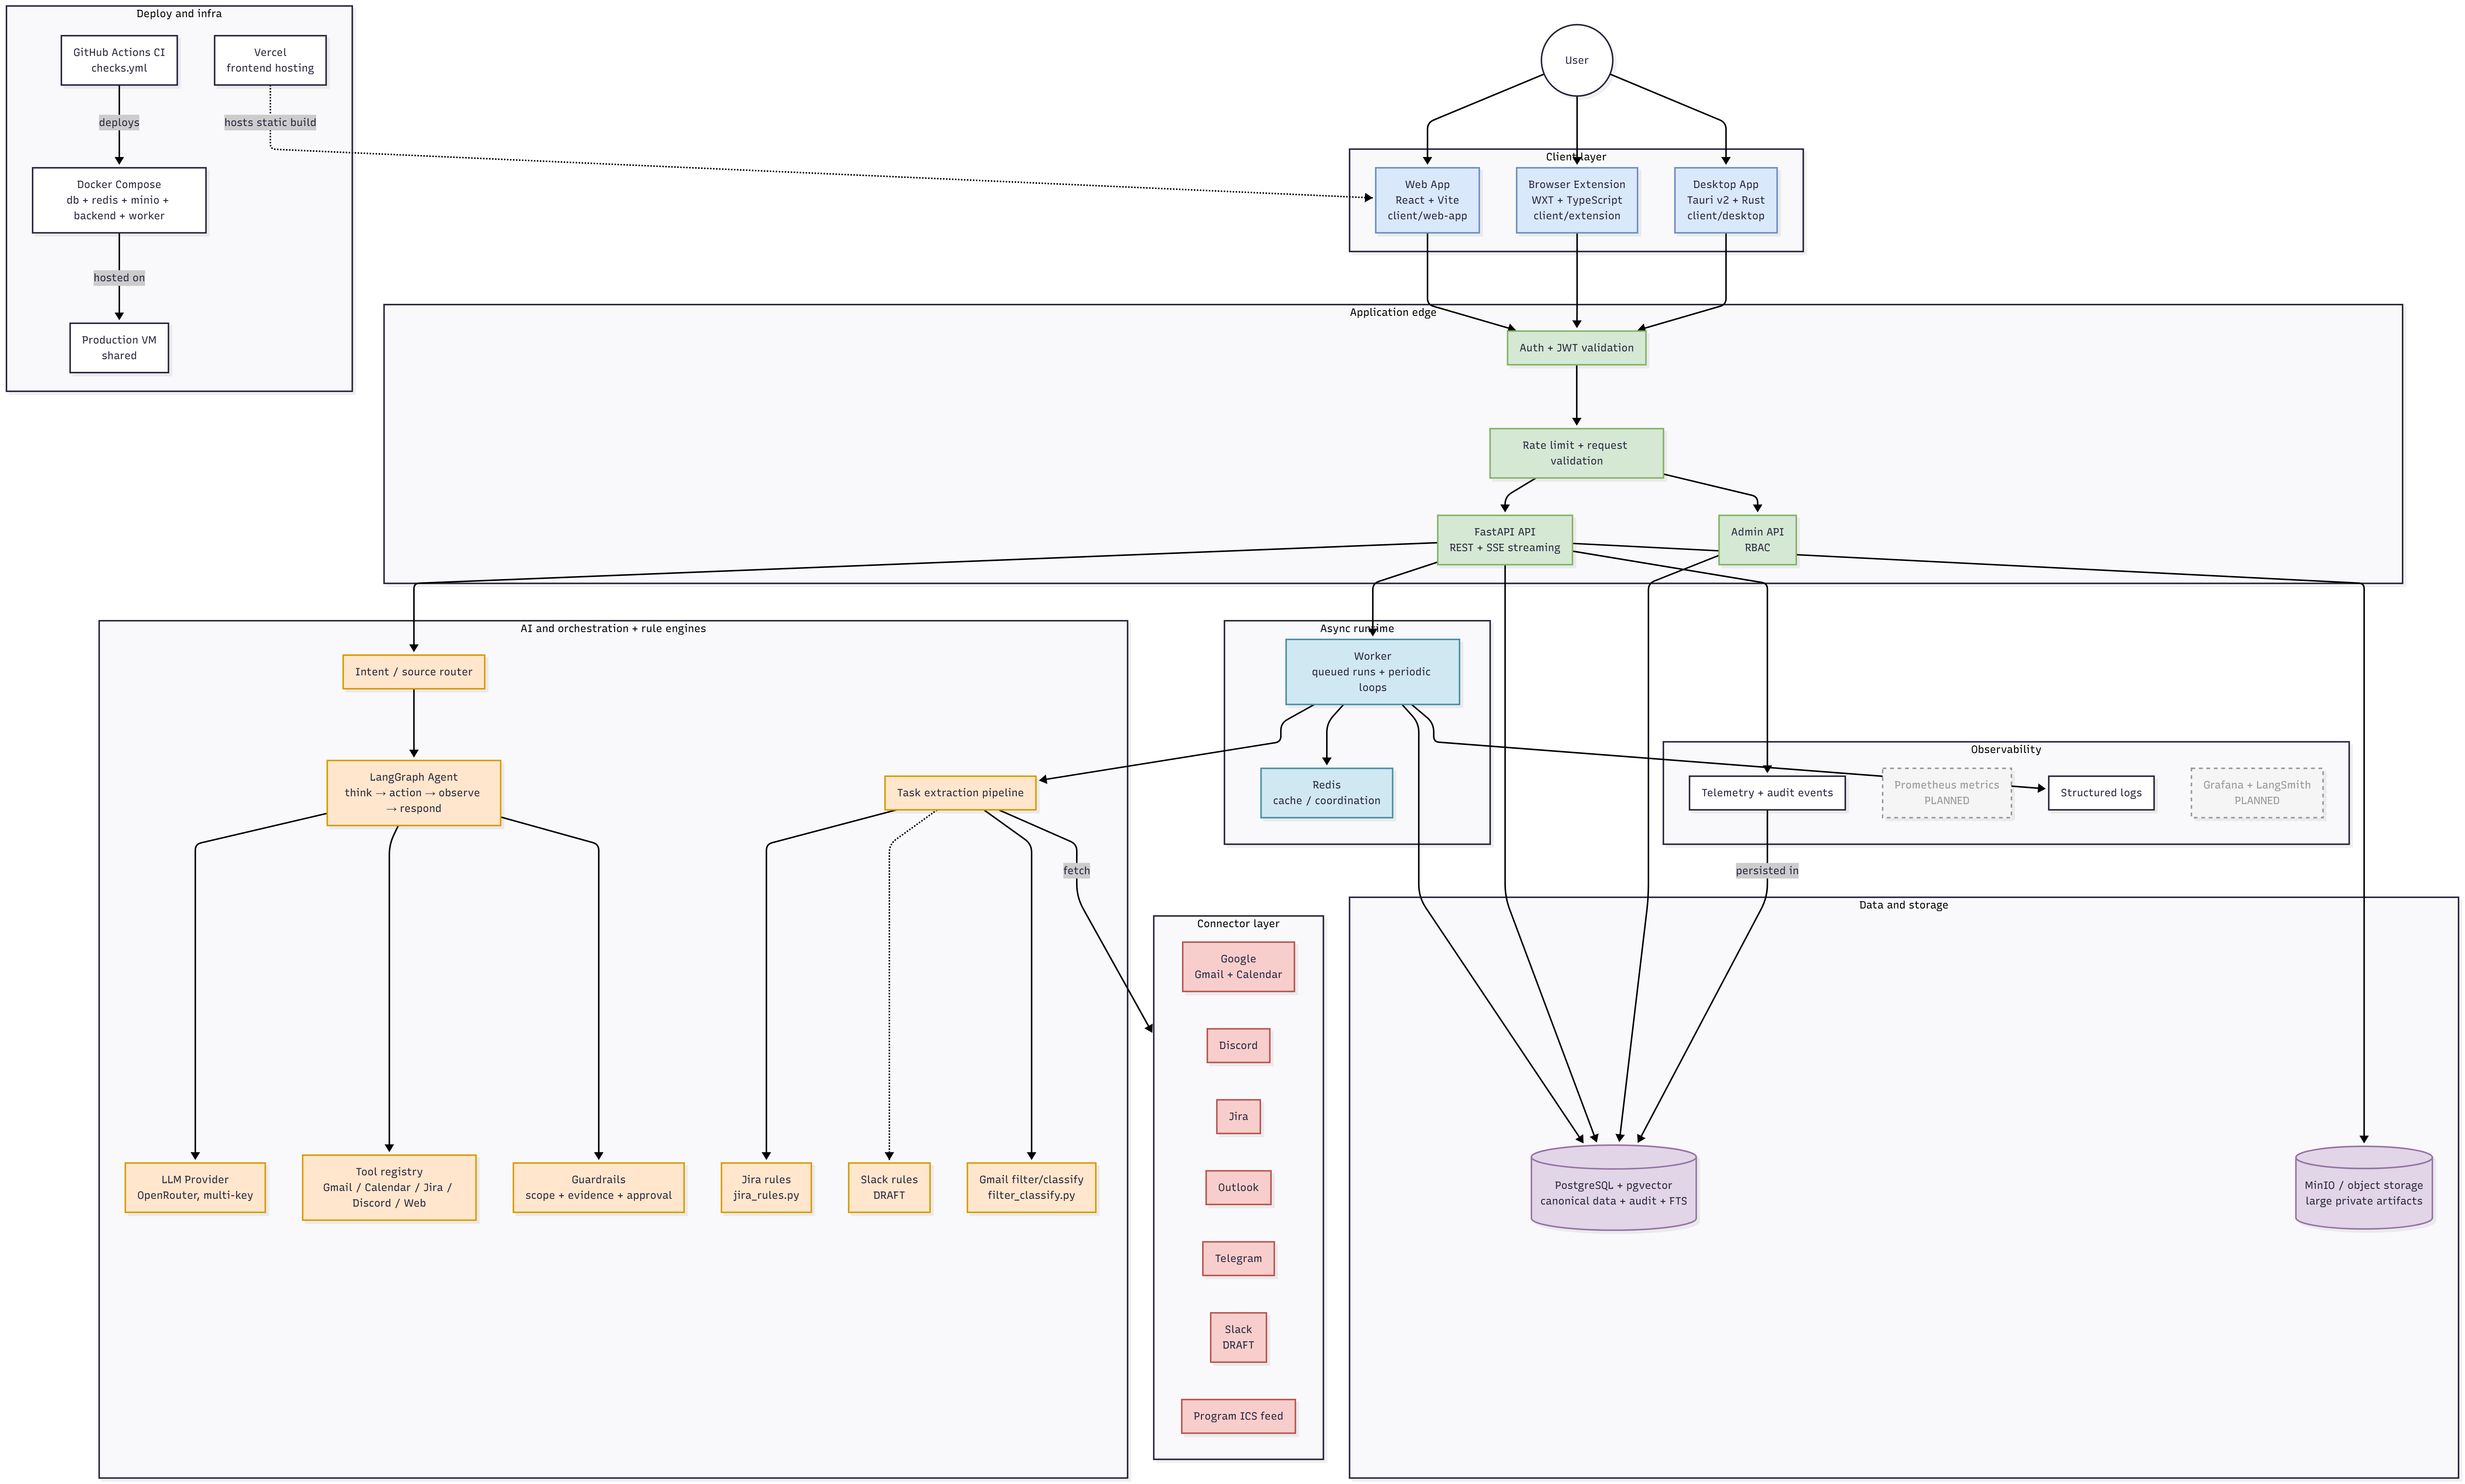
\includegraphics[width=\textwidth]{components/overview.png}
\caption{System context và high-level component topology, dùng trực tiếp từ Gate 2.}
\label{fig:sdd-system-context}
\end{figure}
User chỉ tương tác với web/mobile/extension. Trust boundary bắt đầu tại API edge:
mọi request phải có session, ownership và scope hợp lệ trước khi chạm dữ liệu,
tool hoặc provider. Connector là boundary duy nhất tới nguồn ngoài; PostgreSQL
là canonical store, còn Redis/worker phục vụ điều phối và xử lý bất đồng bộ.

\section{Thiết kế kiến trúc}
\subsection{Style và đơn vị triển khai}
Kiến trúc hiện tại là modular monolith: FastAPI API edge và Python worker dùng
chung PostgreSQL. Module tách theo domain/path, không phải microservice độc lập.
Docker Compose chạy backend và worker. Web được quản lý như frontend riêng;
mobile có project riêng; extension có project WXT/TypeScript riêng.

\begin{longtable}{p{3cm}p{4cm}p{7cm}}
\toprule Unit & Vị trí & Trách nhiệm và ranh giới \\ \midrule
\endhead
Web client & \texttt{client/web-app/} & Onboarding, source, briefing, ask, task/calendar và privacy UI. Không giữ OAuth/provider secret và không gọi LLM/connector trực tiếp. \\
Mobile client & \texttt{apps/mobile/} & Mobile workspace, chat session, file import, widget sync và share intent. Native widget chỉ có giá trị khi chạy native build. \\
Browser extension & \texttt{client/extension/} & UI/notification bề mặt phụ. Không là authoritative data store và không bypass API. \\
Backend API & \texttt{src/main.py}, \texttt{src/api/} & Router FastAPI, Pydantic validation, authentication, HTTP/SSE contract, authorization dependency. Không chạy pipeline dài trong request handler. \\
Worker & \texttt{src/worker.py} & Thực thi sync run và background loop; process dài tách khỏi HTTP request. \\
Data and operations & \texttt{src/models/}, \texttt{alembic/}, \texttt{observability/}, \texttt{scripts/} & Schema, migration, telemetry, health check, deploy và rollback evidence. \\
\bottomrule
\end{longtable}

\subsection{Sơ đồ kiến trúc chuẩn}
Không tạo sơ đồ mới khác Gate 2. Khi review architecture, sử dụng chính xác các
file sau dưới \texttt{docs/projects/gates/gate-2/diagram/}: 
\texttt{components/overview.png} cho toàn cảnh;
\texttt{components/components.png} cho component;
\texttt{data\_flow/full.png} cho end-to-end data/action flow;
\texttt{agent\_flow/agent\_flow.png} cho pipeline;
\texttt{schema/ERD.png}, \texttt{schema/agent\_schema.png},
\texttt{schema/tool\_schema.png} cho schema; và
\texttt{contact/api\_contact.png} cho API boundary.

\begin{figure}[H]
\centering
\includegraphics[width=0.98\textwidth]{components/components.png}
\caption{Phân rã component triển khai, dùng trực tiếp từ Gate 2.}
\label{fig:sdd-components}
\end{figure}

\section{Thiết kế component chi tiết}
\begin{longtable}{p{3cm}p{4.5cm}p{6.5cm}}
\toprule Component & Code chính & Contract thực thi \\ \midrule
\endhead
Identity and access & \texttt{services/auth.py}, \texttt{api/deps.py}, \texttt{services/scope.py} & Backend xác thực session/JWT; object read/write phải qua ownership/source-scope check. Quyền không do model hoặc client quyết định. \\
Connection and connector & \texttt{src/connectors/}, \texttt{services/connections/} & Adapter cho Gmail, Calendar, Discord, Jira, Outlook, Slack, Google Drive/Docs/Sheets. Quản lý token, bounded fetch, pagination/checkpoint và normalize external payload. \\
Evidence and retrieval & \texttt{models/evidence.py}, \texttt{services/retrieval.py}, \texttt{services/attribution.py} & Lưu provenance; retrieval lọc permission trước khi FTS/vector search; answer factual có citation hoặc báo thiếu evidence. \\
Pipeline and run & \texttt{src/agents/pipeline/}, \texttt{models/run.py}, \texttt{models/run\_node\_event.py} & Fetch → normalize → filter → extract → resolve → persist. Run lưu state, count và error; không báo completed khi source bị blocked. \\
Agent and tool & \texttt{src/agents/graph.py}, \texttt{src/agents/tools/}, \texttt{services/llm.py}, \texttt{services/llm\_routing.py} & Route query, select tool/model capability, tool call, observation và response/draft. Tool dùng authenticated scope, không tự cấp quyền. \\
Action domain & \texttt{api/tasks.py}, \texttt{api/calendar.py}, \texttt{services/calendar\_handoff.py}, reminder services & Tạo task/event/reminder proposal; preview, edit, confirm, idempotency và audit. \\
Guardrail & \texttt{src/guardrail/} & Input, output, PII, attachment, policy, query và HITL guard. Source/attachment luôn là input không tin cậy. \\
Observability & \texttt{src/observability.py}, \texttt{src/langsmith_tracing.py}, \texttt{observability/} & Structured telemetry, LangSmith tracing, Prometheus/Grafana dashboards và redaction. \\
\bottomrule
\end{longtable}

\subsection{Context engine và pipeline run}
\begin{figure}[H]
\centering
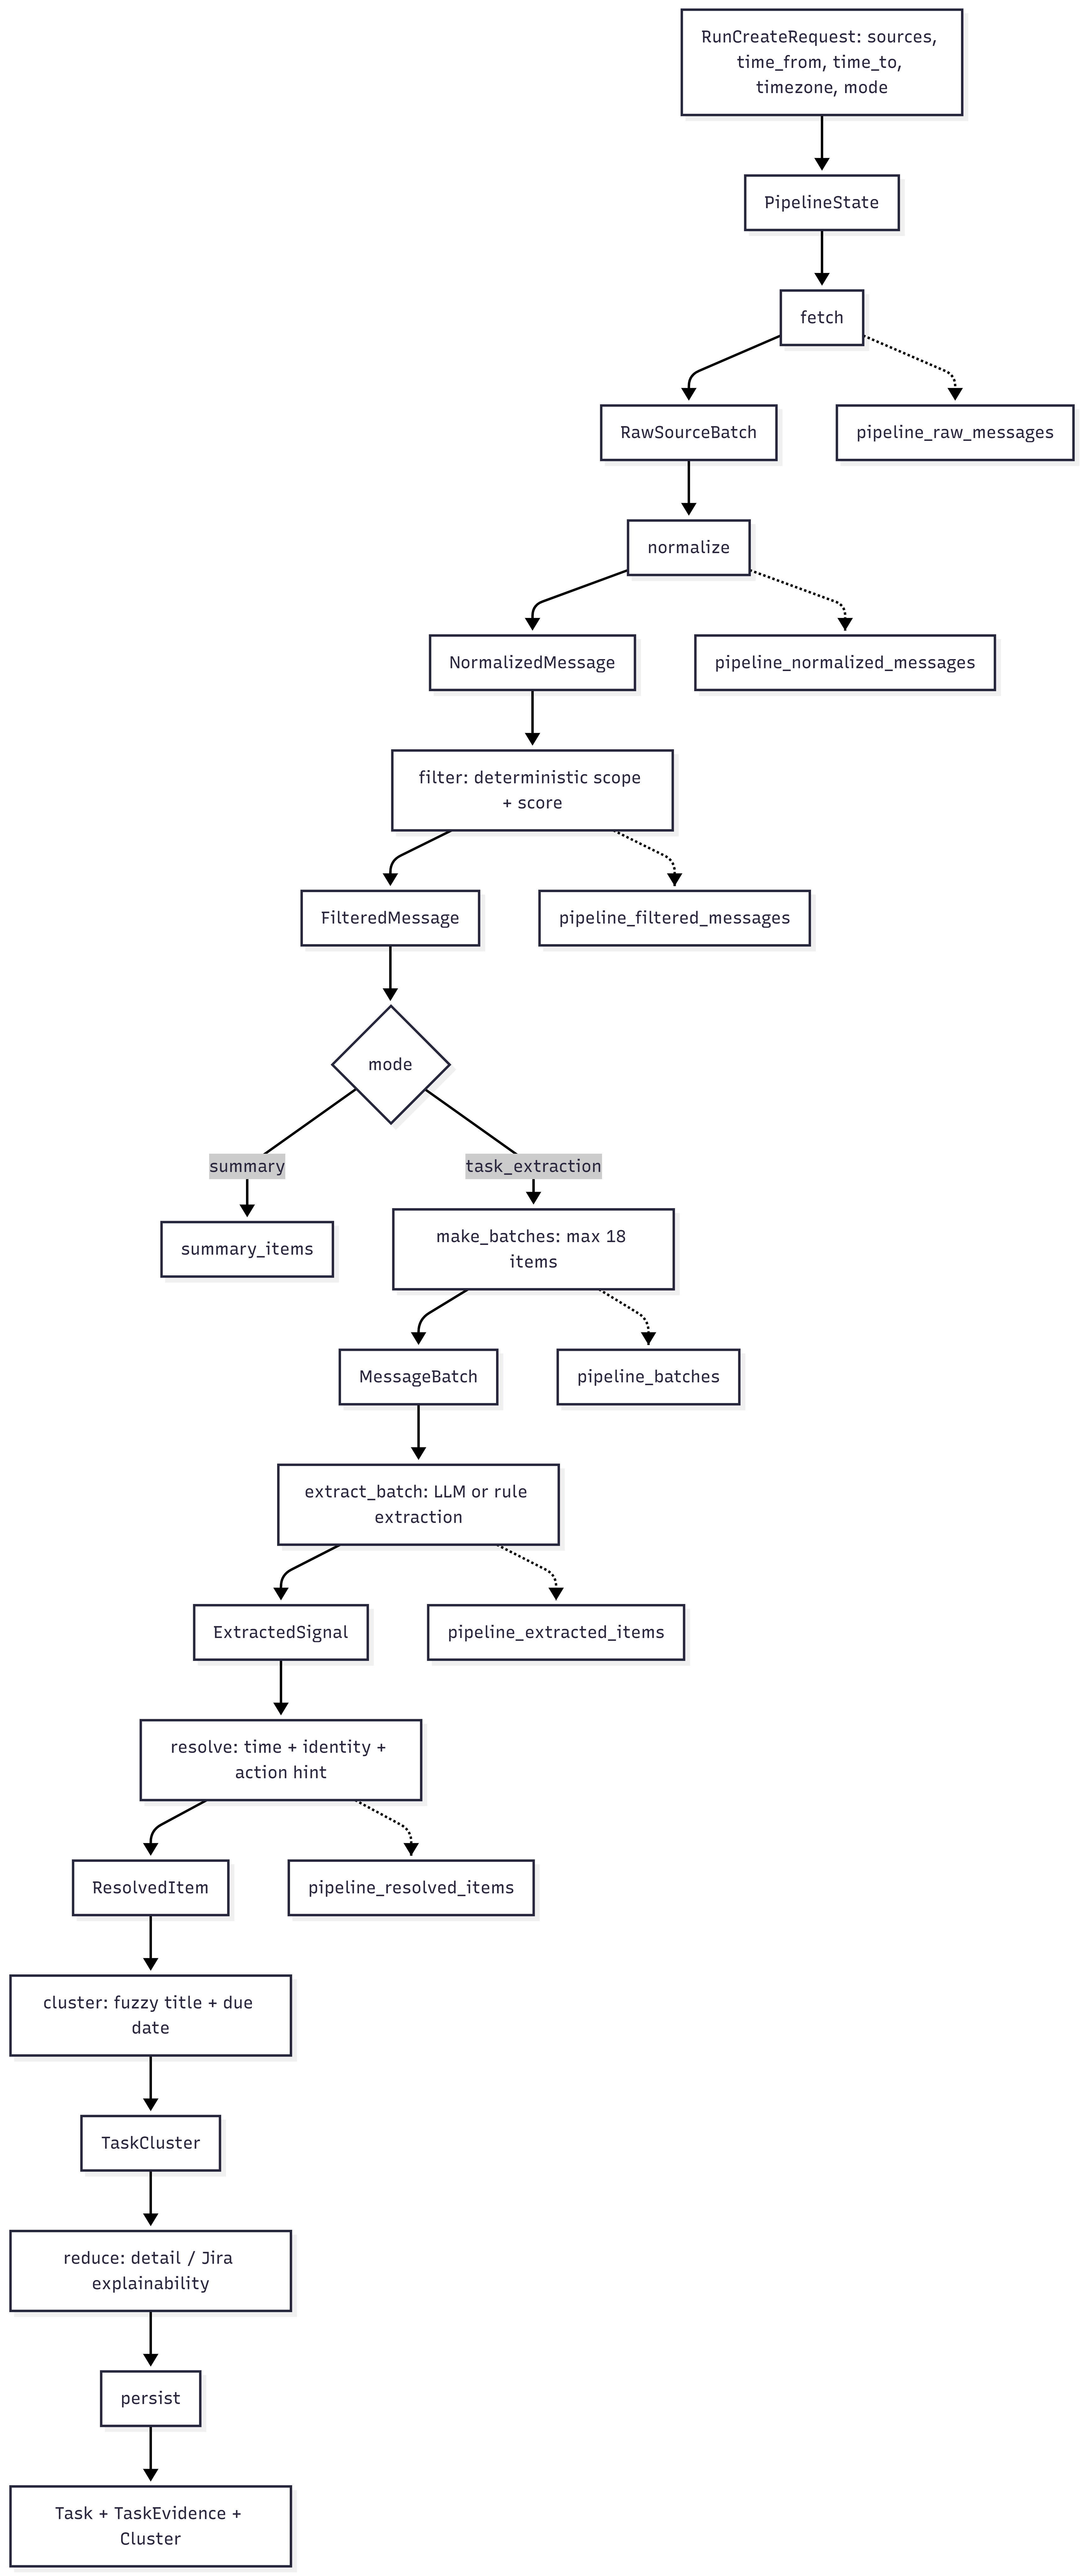
\includegraphics[width=0.96\textwidth]{agent_flow/agent_flow.png}
\caption{Pipeline fetch--normalize--filter--extract--resolve--persist của Context Engine.}
\label{fig:sdd-context-engine}
\end{figure}
\textbf{Input:} source connection, checkpoint/cursor, user scope, time range và
pipeline mode. \textbf{Processing:} connector lấy dữ liệu có giới hạn; pipeline
chuẩn hóa source payload, lọc theo scope/policy, deduplicate, trích task/fact,
resolve entity/deadline và ghi evidence/task/run event. \textbf{Output:} evidence
versioned, task/proposal, coverage, counts và một run state
\code{completed|blocked|failed}. Một source lỗi chỉ làm coverage partial/unknown,
không được biến toàn run thành success giả.

\subsection{Task, planning và calendar action}
Task domain nhận task từ connector, chat, meeting note hoặc file import. Task
giữ title, detail, expected output, context, constraint, execution instruction,
priority, deadline, assignee/stakeholder và evidence link. Planning service dùng
task đã scope-filter, calendar availability, routine/preference và schedule
conflict để tạo recommendation/plan. Calendar/action service chỉ nhận
\code{ActionDraft}: client preview/edit $\rightarrow$ explicit confirm
$\rightarrow$ idempotent handoff $\rightarrow$ audit. Draft bị cancel, missing
field, conflict hoặc provider error không được tạo external event.

\subsection{Interface giữa component}
\begin{longtable}{p{3.2cm}p{3.8cm}p{4.2cm}p{3.1cm}}
\caption{Contract nội bộ quan trọng}\label{tab:sdd-internal-contract}\\
\toprule Caller & Callee & Input tối thiểu & Output/ràng buộc \\ \midrule
\endfirsthead
\toprule Caller & Callee & Input tối thiểu & Output/ràng buộc \\ \midrule
\endhead
API/worker & Connector & user, connection, scope, cursor, time bound & normalized item hoặc typed failure; không trả token cho client. \\
Pipeline & Evidence/retrieval & normalized item, provenance, user scope & version/chunk/citation candidate; replay không duplicate. \\
Agent & Tool registry & authenticated scope, tool schema, request ID & result/error state; tool không tự mở rộng quyền. \\
Agent & Action service & draft payload, confirmation, idempotency key & confirmed handoff/audit hoặc state conflict. \\
UI & API & bearer session, request schema, request ID & DTO/error sanitized; UI không gọi connector/provider. \\
\bottomrule
\end{longtable}

\section{Thiết kế AI và orchestration}
Query router tách lane \texttt{small\_talk} và \texttt{work} theo ADR-005.
Câu mơ hồ đi vào work lane. Work lane chỉ chọn model đã khai báo đúng capability,
đặc biệt tool/function calling khi cần. Failover giữ lane, tool schema, user
scope và trace ID; model không được thay đổi authorization.

Agent thực thi \texttt{think → action → observe → respond}. Tool registry ở
\texttt{src/agents/tools/} gồm Gmail, Calendar, Jira, Drive, Google document,
program information/calendar, task, plan, productivity, time và web search.
Mỗi tool chỉ nhận context đã được backend scope-filter. Tool có khả năng write
chỉ sinh draft/proposal; thao tác ngoài hệ thống cần HITL confirmation.

Input gửi provider được tối thiểu hóa sau consent. Prompt/tool schema được
version cùng code. Trace chỉ cần route lane, model/provider, fallback reason,
latency, usage/cost; không log secret, OAuth token hay raw private source.

\subsection{AI pipeline và structured output}
\begin{figure}[H]
\centering
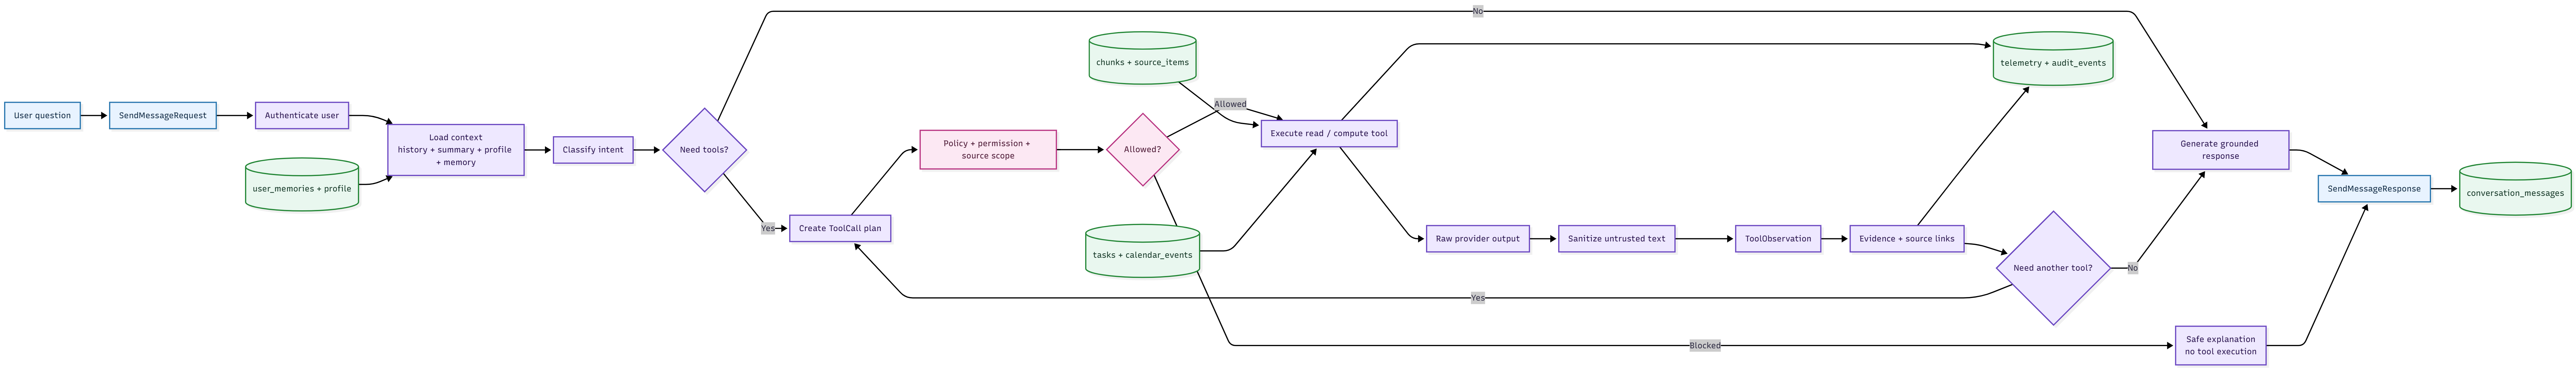
\includegraphics[width=0.96\textwidth]{data_flow/agent.png}
\caption{Luồng agent từ request, scope/tool policy đến answer hoặc draft.}
\label{fig:sdd-ai-pipeline}
\end{figure}
Mỗi request work đi qua: (1) validate session/AI consent; (2) deterministic
intent/source route; (3) retrieval evidence đã permission-filter; (4) tool plan
và execution có guard; (5) response validator; (6) answer, abstain, conflict
hoặc action draft. Structured output tối thiểu có \code{answer\_kind},
\code{content}, \code{citations}, \code{coverage}, \code{requires\_confirmation}
và \code{tool\_outcome}. Validator từ chối response có factual claim không có
evidence, claim trái tool result hoặc action chưa confirm.

\subsection{Model, prompt và guardrail}
Provider/model nằm trong centralized configuration, không hard-code ở UI/tool.
Prompt system định nghĩa role hỗ trợ, evidence-only factual answer, không đoán
deadline/owner, yêu cầu báo conflict/coverage và cấm external write. Temperature,
max token, tool schema, prompt version, provider/model và fallback reason phải
vào trace. Guardrail input kiểm PII/attachment/prompt injection; guardrail query
kiểm scope/time range; guardrail output kiểm citation, policy và action state.

\subsection{AI failure policy}
Nếu retrieval rỗng, answer là abstain/clarify. Nếu tool bị 401/403/revoked,
answer nêu permission/source unavailable. Nếu tool timeout/429/5xx, worker hoặc
agent retry có giới hạn/failover đúng capability lane; nếu hết candidate thì trả
error rõ. Không fallback sang model không có tool capability cho work request.

\section{Thiết kế dữ liệu}
PostgreSQL/SQLAlchemy và Alembic là schema authority. ERD review nằm ở
\texttt{gate-2/diagram/schema/ERD.png}. Các aggregate thực tế gồm:
\begin{figure}[H]
\centering
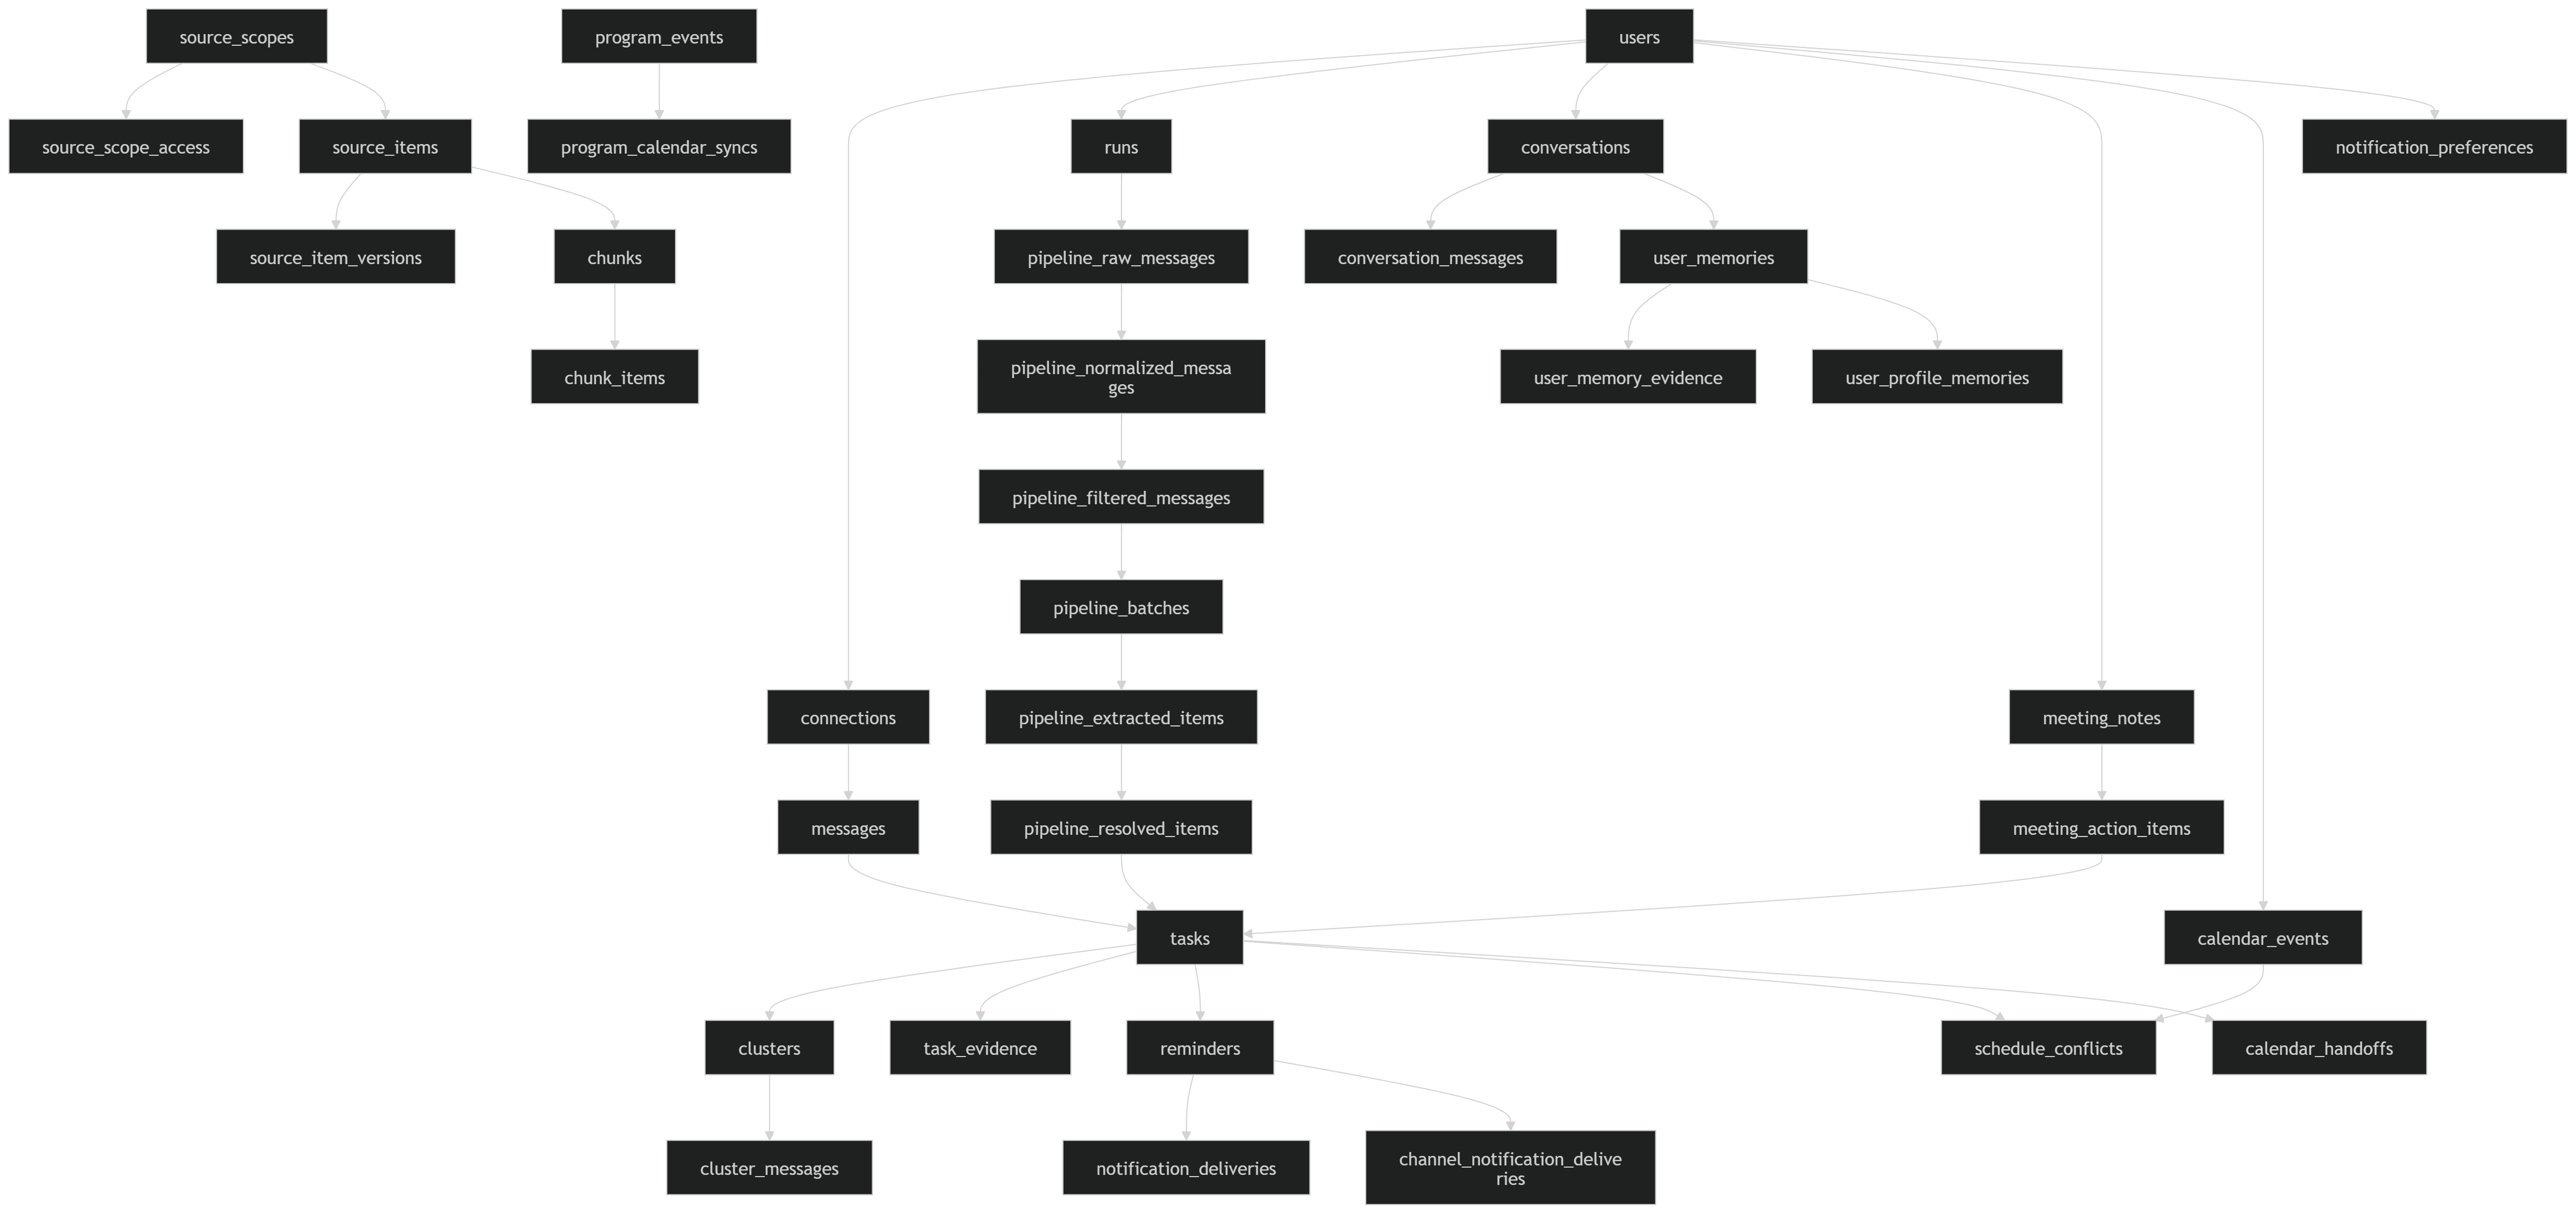
\includegraphics[width=0.98\textwidth]{schema/ERD.png}
\caption{ERD canonical: identity, source/evidence, run, task, calendar và conversation.}
\label{fig:sdd-erd}
\end{figure}
\begin{longtable}{p{3.2cm}p{4.3cm}p{6.5cm}}
\toprule Aggregate & Models/dữ liệu & Invariant \\ \midrule
\endhead
Identity and source access & user, connection, source scope access, sync cursor & Connection/scope thuộc user; revoke/pause ngăn ingest và retrieval mới. \\
Evidence & evidence, document read, source metadata/version/chunk & Lưu source identity, provenance và thời điểm; không dùng cache để vượt permission. \\
Run and audit & run, run node event, pipeline audit, worker heartbeat, telemetry & Mỗi run có lifecycle/count/error; telemetry không mang raw private content. \\
Task and schedule & task, task evidence, reminder, calendar event/handoff, schedule conflict & Task/action có evidence/audit; external write chỉ sau confirmation. \\
Conversation and memory & conversation, message, user memory, learning, rating & Memory/answer phải chịu scope; feedback/rating hỗ trợ evaluation. \\
\bottomrule
\end{longtable}
Migration mới phải nêu forward step, backfill/compatibility, rollback và restore
test. Retention, RPO và RTO chưa được code/ADR chốt không được biến thành claim.

\subsection{Schema contract mức entity}
\begin{longtable}{p{3.0cm}p{3.5cm}p{3.0cm}p{4.7cm}}
\caption{Field và constraint phải giữ khi thay đổi schema}\label{tab:sdd-schema-contract}\\
\toprule Entity & Field chính & Kiểu logic & Constraint/ý nghĩa \\ \midrule
\endfirsthead
\toprule Entity & Field chính & Kiểu logic & Constraint/ý nghĩa \\ \midrule
\endhead
User & id, email, role & UUID/string/enum & ID là owner boundary; identity không vào telemetry không cần thiết. \\
Connection & user\_id, provider, token metadata, status & FK/enum/json & Thuộc một user; token server-side; revoked chặn ingest. \\
Evidence & id, user\_id, source identity, provenance, content/time & UUID/FK/json/text/time & Có provenance/version; retrieval scope-filter trước. \\
Run & id, state, counts, error class, request ID & UUID/enum/json/string & State completed/blocked/failed; count phản ánh outcome thật. \\
Task & id, user\_id, title, priority, due\_at, status & UUID/FK/text/enum/time & Task thuộc user; evidence/audit giữ nguyên nhân proposal. \\
Action draft & id, payload, state, idempotency key & UUID/json/enum/string & Confirmed mới handoff; key trùng payload khác là conflict. \\
Conversation/message & conversation\_id, user\_id, role, content & FK/FK/enum/text & Context không vượt user scope; factual output liên kết citation. \\
\bottomrule
\end{longtable}

\section{Thiết kế tích hợp}
\begin{longtable}{p{3cm}p{4cm}p{7cm}}
\toprule Tích hợp & Boundary code & Failure/safety behavior \\ \midrule
\endhead
OAuth source & Connector và connection service & Token server-side; scope tối thiểu; bounded polling/webhook; checkpoint, retry/backoff và revoke. \\
LLM provider & LLM routing/service & Capability-aware candidate selection; retry/failover có giới hạn; schema error không retry mù; hết candidate trả error/abstain. \\
Calendar handoff & Calendar service, ICS/handoff adapter & Hệ thống tạo draft/preview; confirmed mới handoff/write; provider unavailable dùng handoff/template phù hợp. \\
Notification & Web push, Telegram/Discord channel services & Delivery state/audit; lỗi delivery không chuyển nghiệp vụ thành completed. \\
File intake & Attachment extract, spreadsheet task extraction, mobile file import & Allowlist type/size, timeout, file close; attachment là untrusted input. \\
\bottomrule
\end{longtable}
Mọi thay đổi sync/brief/agent/task/action phải đối chiếu lần lượt các sơ đồ
\texttt{data\_flow/sync.png}, \texttt{brief.png}, \texttt{agent.png},
\texttt{task.png}, \texttt{action.png} của Gate 2.

\begin{figure}[H]
\centering
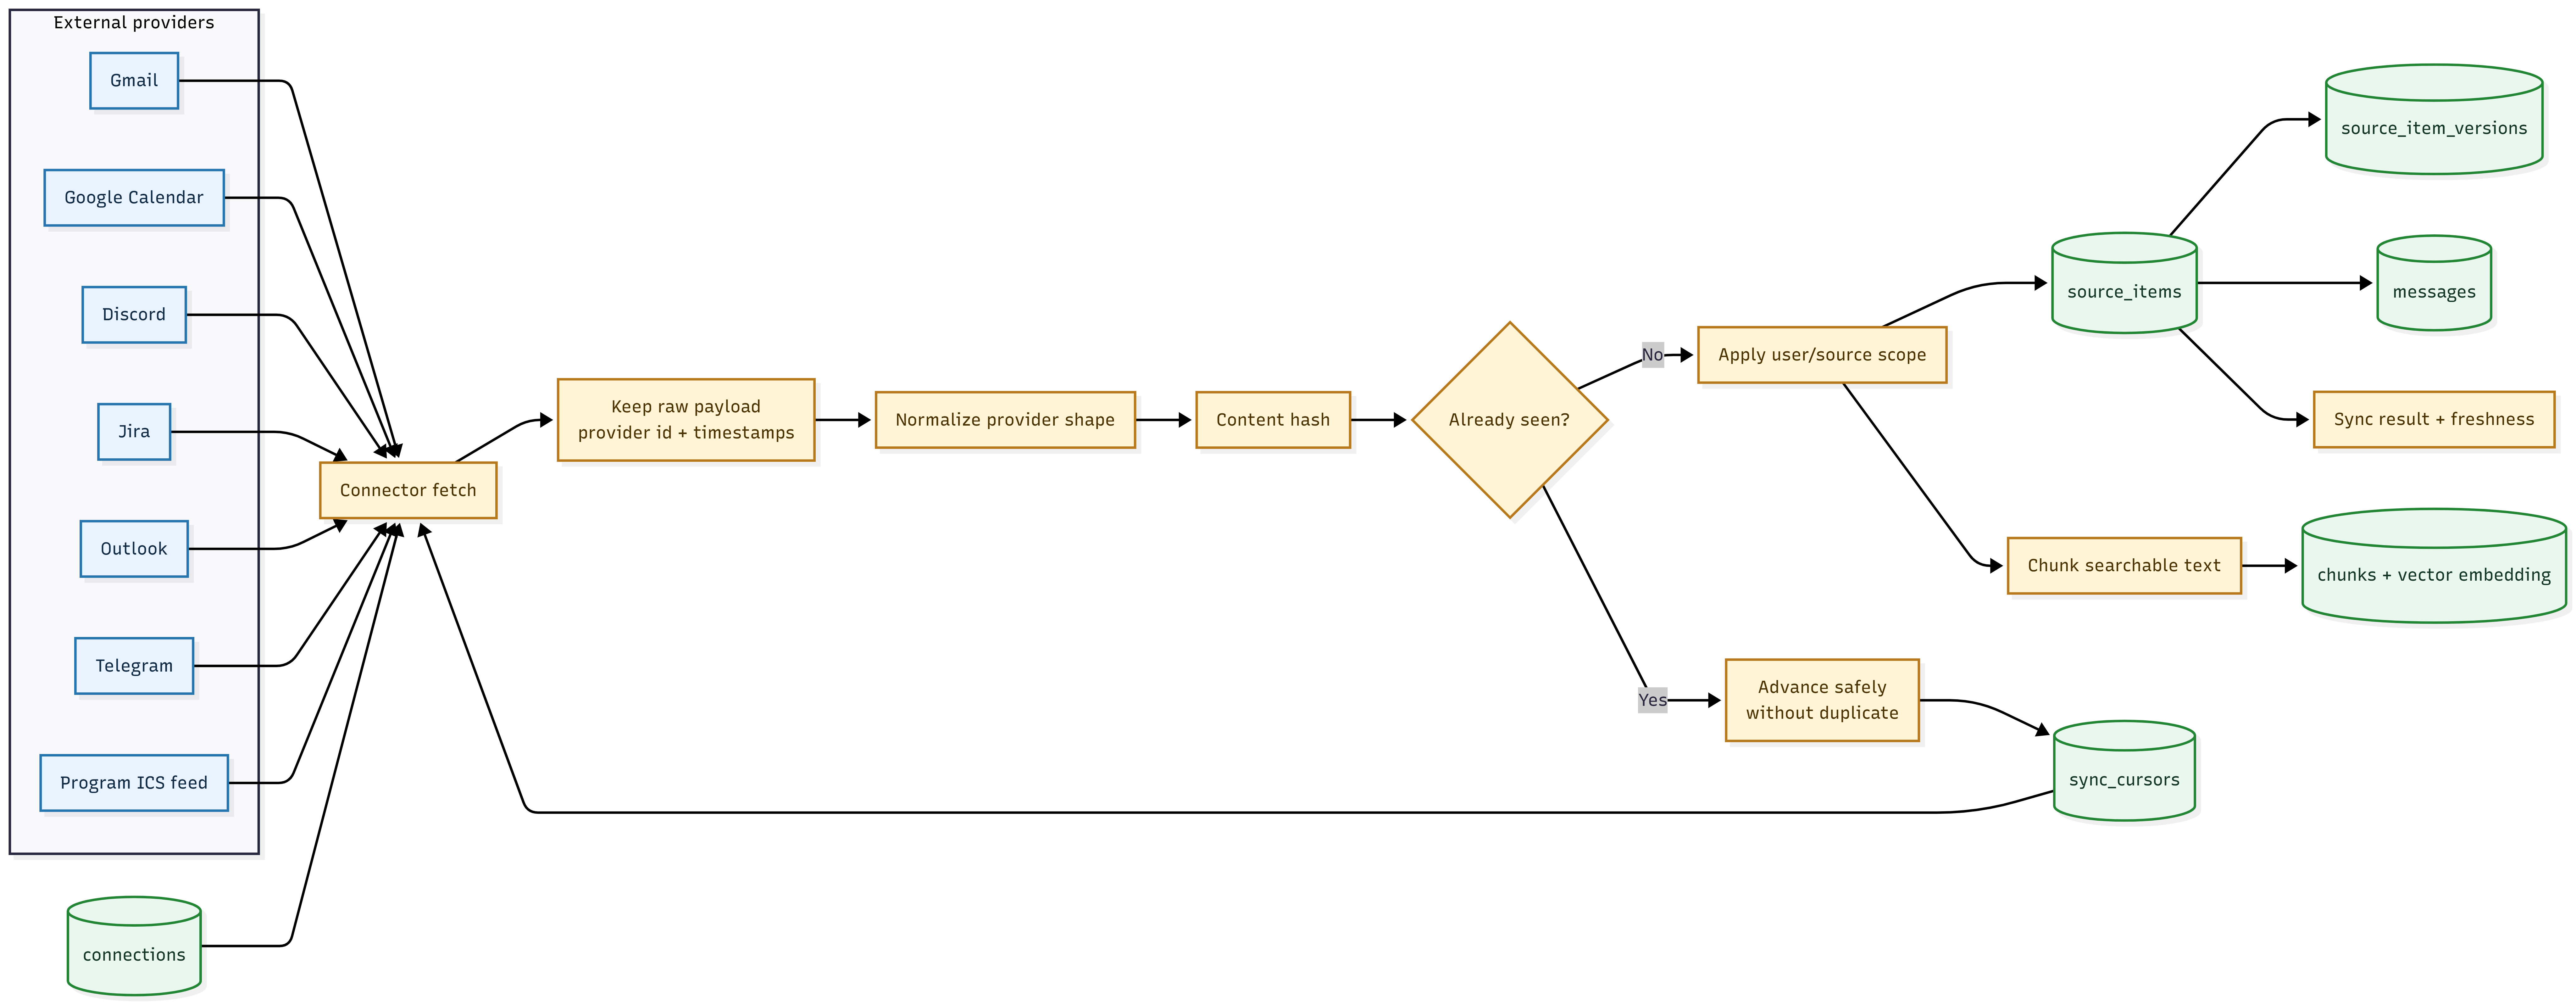
\includegraphics[width=0.96\textwidth]{data_flow/sync.png}
\caption{Thiết kế sync: source connector, normalize, evidence và run receipt.}
\label{fig:sdd-sync}
\end{figure}

\subsection{Connector contract theo provider}
\begin{longtable}{p{2.7cm}p{3.4cm}p{4.2cm}p{3.9cm}}
\caption{Thiết kế tích hợp nguồn công việc}\label{tab:sdd-provider-contract}\\
\toprule Provider/nhóm & Capability trong code & Mapping vào domain & Error/retry/revoke \\ \midrule
\endfirsthead
\toprule Provider/nhóm & Capability trong code & Mapping vào domain & Error/retry/revoke \\ \midrule
\endhead
Gmail/Outlook & Search/read thread/message, connector state & Email/evidence, deadline/action candidate, citation & OAuth expiry/refresh lỗi $\rightarrow$ blocked; giữ checkpoint, không báo coverage complete. \\
Google Calendar & Search event, calendar cache/handoff, conflict & Calendar event, availability, reminder, action draft & Rate limit/timeout retry bounded; write chỉ sau confirm/idempotency. \\
Jira & Search issue, rule/service, project context & Issue/task, assignee, due date, project evidence & Scope/permission denial không lộ issue metadata; source unavailable là partial coverage. \\
Discord/Slack/Telegram & Channel/message/thread delivery & Message evidence, channel notification/shared chat & Channel delivery audit; lỗi delivery không đổi state task/action. \\
Drive/Docs/Sheets/File & Picker, document read, spreadsheet extraction & Document evidence, task proposal, attachment & MIME/size/timeout validation; attachment treated untrusted. \\
\bottomrule
\end{longtable}

\section{Thiết kế API}
Các router được gắn dưới \texttt{/api/v1} tại \texttt{src/main.py}: auth,
connections, conversations, tasks, calendar, reminders, routines, runs, memory,
meeting notes, integrations, intent, Google Drive/Docs/Sheets, Excel import,
ratings, push, channels và admin. Request dùng bearer token trừ auth bootstrap.
API trả correlation/request ID, timestamp timezone-aware và error sanitized:
\begin{center}
\texttt{\{error: \{code, message, details, request\_id\}\}}.
\end{center}
Các endpoint write nhận idempotency behavior phù hợp. Contract test luôn bao gồm
success path, unauthenticated, unauthorized/cross-user, invalid input, expired/
revoked connection và retry/state conflict khi endpoint có side effect.

\subsection{Nhóm API và contract}
\begin{longtable}{p{3.4cm}p{3.2cm}p{4.1cm}p{3.5cm}}
\caption{Catalogue API theo bounded capability}\label{tab:sdd-api-catalogue}\\
\toprule Nhóm & Router & Request/response chính & Validation/error \\ \midrule
\endfirsthead
\toprule Nhóm & Router & Request/response chính & Validation/error \\ \midrule
\endhead
Identity/connection & auth, connections, integrations & Session, OAuth start/callback, connection state & 401/403, expiry/revoke, ownership, sanitized provider error. \\
Conversation/agent & conversations, messages, intent, memory, public ask & query/message, stream event, citation, tool outcome & Scope/consent, SSE error event, abstain/coverage, provider timeout. \\
Task/planning/calendar & tasks, calendar, routines, reminders, schedule conflicts & task/action draft, plan, event preview, confirmation & Required field, timezone, state conflict, idempotency, no write before confirm. \\
Evidence/import/run & runs, Drive/Docs/Sheets, excel, storage & source/file selection, run receipt, task proposal & MIME/size, revoked connection, retry/duplicate, blocked outcome. \\
Product/admin/channel & meeting notes, ratings, push, channels, projects, admin & note, feedback, subscription, program/project DTO & Role check, delivery state, no raw private data in telemetry. \\
\bottomrule
\end{longtable}

\subsection{Ví dụ action draft contract}
\textbf{Request} từ UI gửi \code{Idempotency-Key}, session và payload draft:
\begin{verbatim}
POST /api/v1/calendar/action-drafts/{id}/confirm
{
  "confirmation": true,
  "timezone": "Asia/Bangkok"
}
\end{verbatim}
\textbf{Response} trả state đã confirm/handoff, citation/evidence reference,
request ID và error code nếu conflict. Nếu \code{confirmation=false}, missing
mandatory field, scope invalid hoặc key trùng với payload khác, backend không gọi
provider write và trả 400/403/409 theo error contract.

\section{Thiết kế UI/UX}
Nhi phụ trách UI/UX; nguồn chuẩn là \texttt{docs/projects/design/wireframe-ui-flow.md}
và Figma được liên kết trong tài liệu đó. UI web/mobile/extension chỉ dùng API,
không cất system secret và không gọi provider/connector trực tiếp.

Các view cần phản ánh contract backend: onboarding/consent/source connection;
briefing/ask/evidence citation; task/calendar/action draft; privacy/audit;
meeting notes; mobile file import/chat/widget. State tối thiểu gồm loading,
empty, connected, paused, revoked, partial coverage, conflict, abstain,
drafted, previewed, confirmed, cancelled, retryable error và denied. Action
preview phải hiển thị timezone; state không chỉ biểu đạt bằng màu; keyboard,
visible focus, semantic label và layout tiếng Việt là bắt buộc.

\subsection{Interface contract theo màn hình}
\begin{longtable}{p{3.0cm}p{3.7cm}p{4.0cm}p{3.5cm}}
\caption{Màn hình quan trọng, data source và interaction boundary}\label{tab:sdd-ui-contract}\\
\toprule Interface & Data/API & Interaction chính & State bắt buộc \\ \midrule
\endfirsthead
\toprule Interface & Data/API & Interaction chính & State bắt buộc \\ \midrule
\endhead
Onboarding/Sources & auth, connections, data privacy & Connect, reconnect, pause, revoke consent & loading, connected, paused, revoked, OAuth error, scope limited. \\
Briefing/Ask & conversations, messages, briefing, evidence & Ask, stream response, open citation, feedback, follow-up & loading, citation, partial/unknown coverage, conflict, abstain, retry. \\
Task/Plan & tasks, projects, routines, schedule conflict & View/edit/approve task, priority/filter, generate/revise plan & empty, proposed, approved, done, overdue, conflict, error. \\
Calendar/Action & calendar, reminders, action handoff & Preview/edit/confirm/cancel event or reminder & drafted, previewed, confirmed, cancelled, handoff failed. \\
Mobile/File/Widget & excel/file intake, chat session, widget sync & Select/share file, review proposal, widget snapshot & validation error, permission denied, keyboard-safe, native-build indicator. \\
Privacy/Audit/Admin & privacy, audit, admin, ratings & Export/delete/revoke, inspect activity, admin configuration & denied, destructive confirmation, redacted audit, retryable error. \\
\bottomrule
\end{longtable}

\section{Thiết kế bảo mật và riêng tư}
\begin{longtable}{p{3.5cm}p{5cm}p{5.5cm}}
\toprule Rủi ro & Control trong code/design & Evidence kiểm chứng \\ \midrule
\endhead
Cross-user access & Auth + ownership/source-scope ở API/service/query; cache permission-scoped; RLS là defence in depth. & Two-user denial và regression test. \\
Secret/token leak & Secret chỉ ở server; OAuth token không trả client; telemetry/error redacted. & Secret/log scan và sanitized-error test. \\
Prompt injection & Attachment/source là untrusted; guardrail + tool allow-list; tool không tăng quyền. & Malicious fixture không vượt scope/HITL. \\
Consent/revoke/delete & Consent AI trước provider call; revoke/delete invalidates evidence/memory/search/brief/answer mới. & Revoke/delete absence test. \\
Unsafe action & Draft-preview-confirm, idempotency, audit. & Không có external write trước explicit confirmation. \\
\bottomrule
\end{longtable}

\subsection{Security boundary và authorization flow}
Mọi request bắt đầu bằng bearer/session validation ở API edge. Service lấy user
identity từ session đã xác thực, không lấy từ payload/model. Trước read/write,
service kiểm object ownership, source scope, consent còn hiệu lực và role khi
đi vào admin route. Connector token và provider key chỉ nằm ở server/runtime
secret store; client chỉ có public configuration/session token. Citation open,
cache và background job đều phải re-check permission hiện tại, vì quyền có thể
bị revoke sau khi response/draft được tạo.

\subsection{Data boundary cho AI}
AI chỉ nhận query và evidence tối thiểu đã scope-filter sau consent. Không gửi
credential, raw token, dữ liệu user khác, attachment không qua safety check hay
source đã revoke. Provider trace được redaction trước khi đi vào LangSmith;
audit giữ request ID, state, model/provider metadata và reason code thay vì raw
private content. Export/delete phải invalidate cache, retrieval index, memory,
briefing và answer mới theo cùng user/source scope.

\section{Xử lý lỗi và độ tin cậy}
Connector timeout/429/revoke dùng retry/backoff có giới hạn, giữ checkpoint và
trả blocked/partial coverage nếu không hoàn tất. Worker restart/duplicate request
dùng durable run + idempotency để tránh mất hoặc nhân bản item. LLM timeout/5xx/
tool failure chỉ failover trong capability lane; lỗi schema không retry mù; hết
candidate trả error/abstain. File/API validation reject sớm, không persist dở
dang. Deploy/migration lỗi dùng health check và rollback artifact; fast path
không restart database, Redis, MinIO hay shared proxy.

\subsection{Failure matrix và recovery contract}
\begin{longtable}{p{3.2cm}p{4.2cm}p{4.0cm}p{3.0cm}}
\caption{Lỗi, trạng thái trả về và recovery}\label{tab:sdd-failure-matrix}\\
\toprule Failure & Detection & Recovery/response & Evidence \\ \midrule
\endfirsthead
\toprule Failure & Detection & Recovery/response & Evidence \\ \midrule
\endhead
OAuth expired/revoked & Provider 401/invalid grant, consent state & Mark connection blocked/revoked; stop new ingest; actionable reconnect UI. & Connection/audit event, no new evidence. \\
Provider timeout/429/5xx & Timeout/rate-limit/error class & Bounded retry/backoff; retain checkpoint; coverage partial/unknown. & Run counts, retry attempt, source freshness. \\
Worker restart/duplicate & Lease/heartbeat/idempotency key & Resume durable run or replay safely; no lost/duplicate item. & Run state, cursor, duplicate regression. \\
LLM/tool failure & Provider/tool result/error taxonomy & Failover compatible candidate or abstain/error; preserve scope/tool binding. & Trace lane/model/fallback/reason. \\
Invalid file/request & Pydantic/MIME/size/schema validation & Reject before persist; return actionable 4xx error. & Request ID, validation code, no partial object. \\
Action conflict/write failure & State/idempotency/provider response & Do not repeat unsafe write; return draft/failed state and allow retry/review. & Action audit, provider handoff ID. \\
\bottomrule
\end{longtable}

SLO tham chiếu SRS: P95 batch/briefing $\leq2$s, first answer $\leq10$s, action
draft $\leq3$s tại tải 50 active users. Báo cáo bắt buộc có environment, sample
size, percentile, failed request và SHA.

\section{Kiến trúc triển khai và quan sát}
Docker Compose chạy backend/worker và các dependency runtime. Theo runbook,
fast path chỉ build/recreate \texttt{p004-backend} và \texttt{worker}; database,
Redis, MinIO và shared proxy không bị restart. Web được Vercel quản lý; mobile
đi qua EAS/TestFlight/native build. Production environment trên VM là
authoritative và không được copy vào Git hoặc test run.

Health endpoint, structured logs, Prometheus/Grafana và LangSmith theo dõi source
freshness, queue age/retry, duplicate rate, run/connector error, LLM lane/model/
fallback, latency, token/cost, citation failure và provider availability. Deploy
chỉ dùng artifact/SHA đã verify, có health evidence và rollback target.

\begin{figure}[H]
\centering
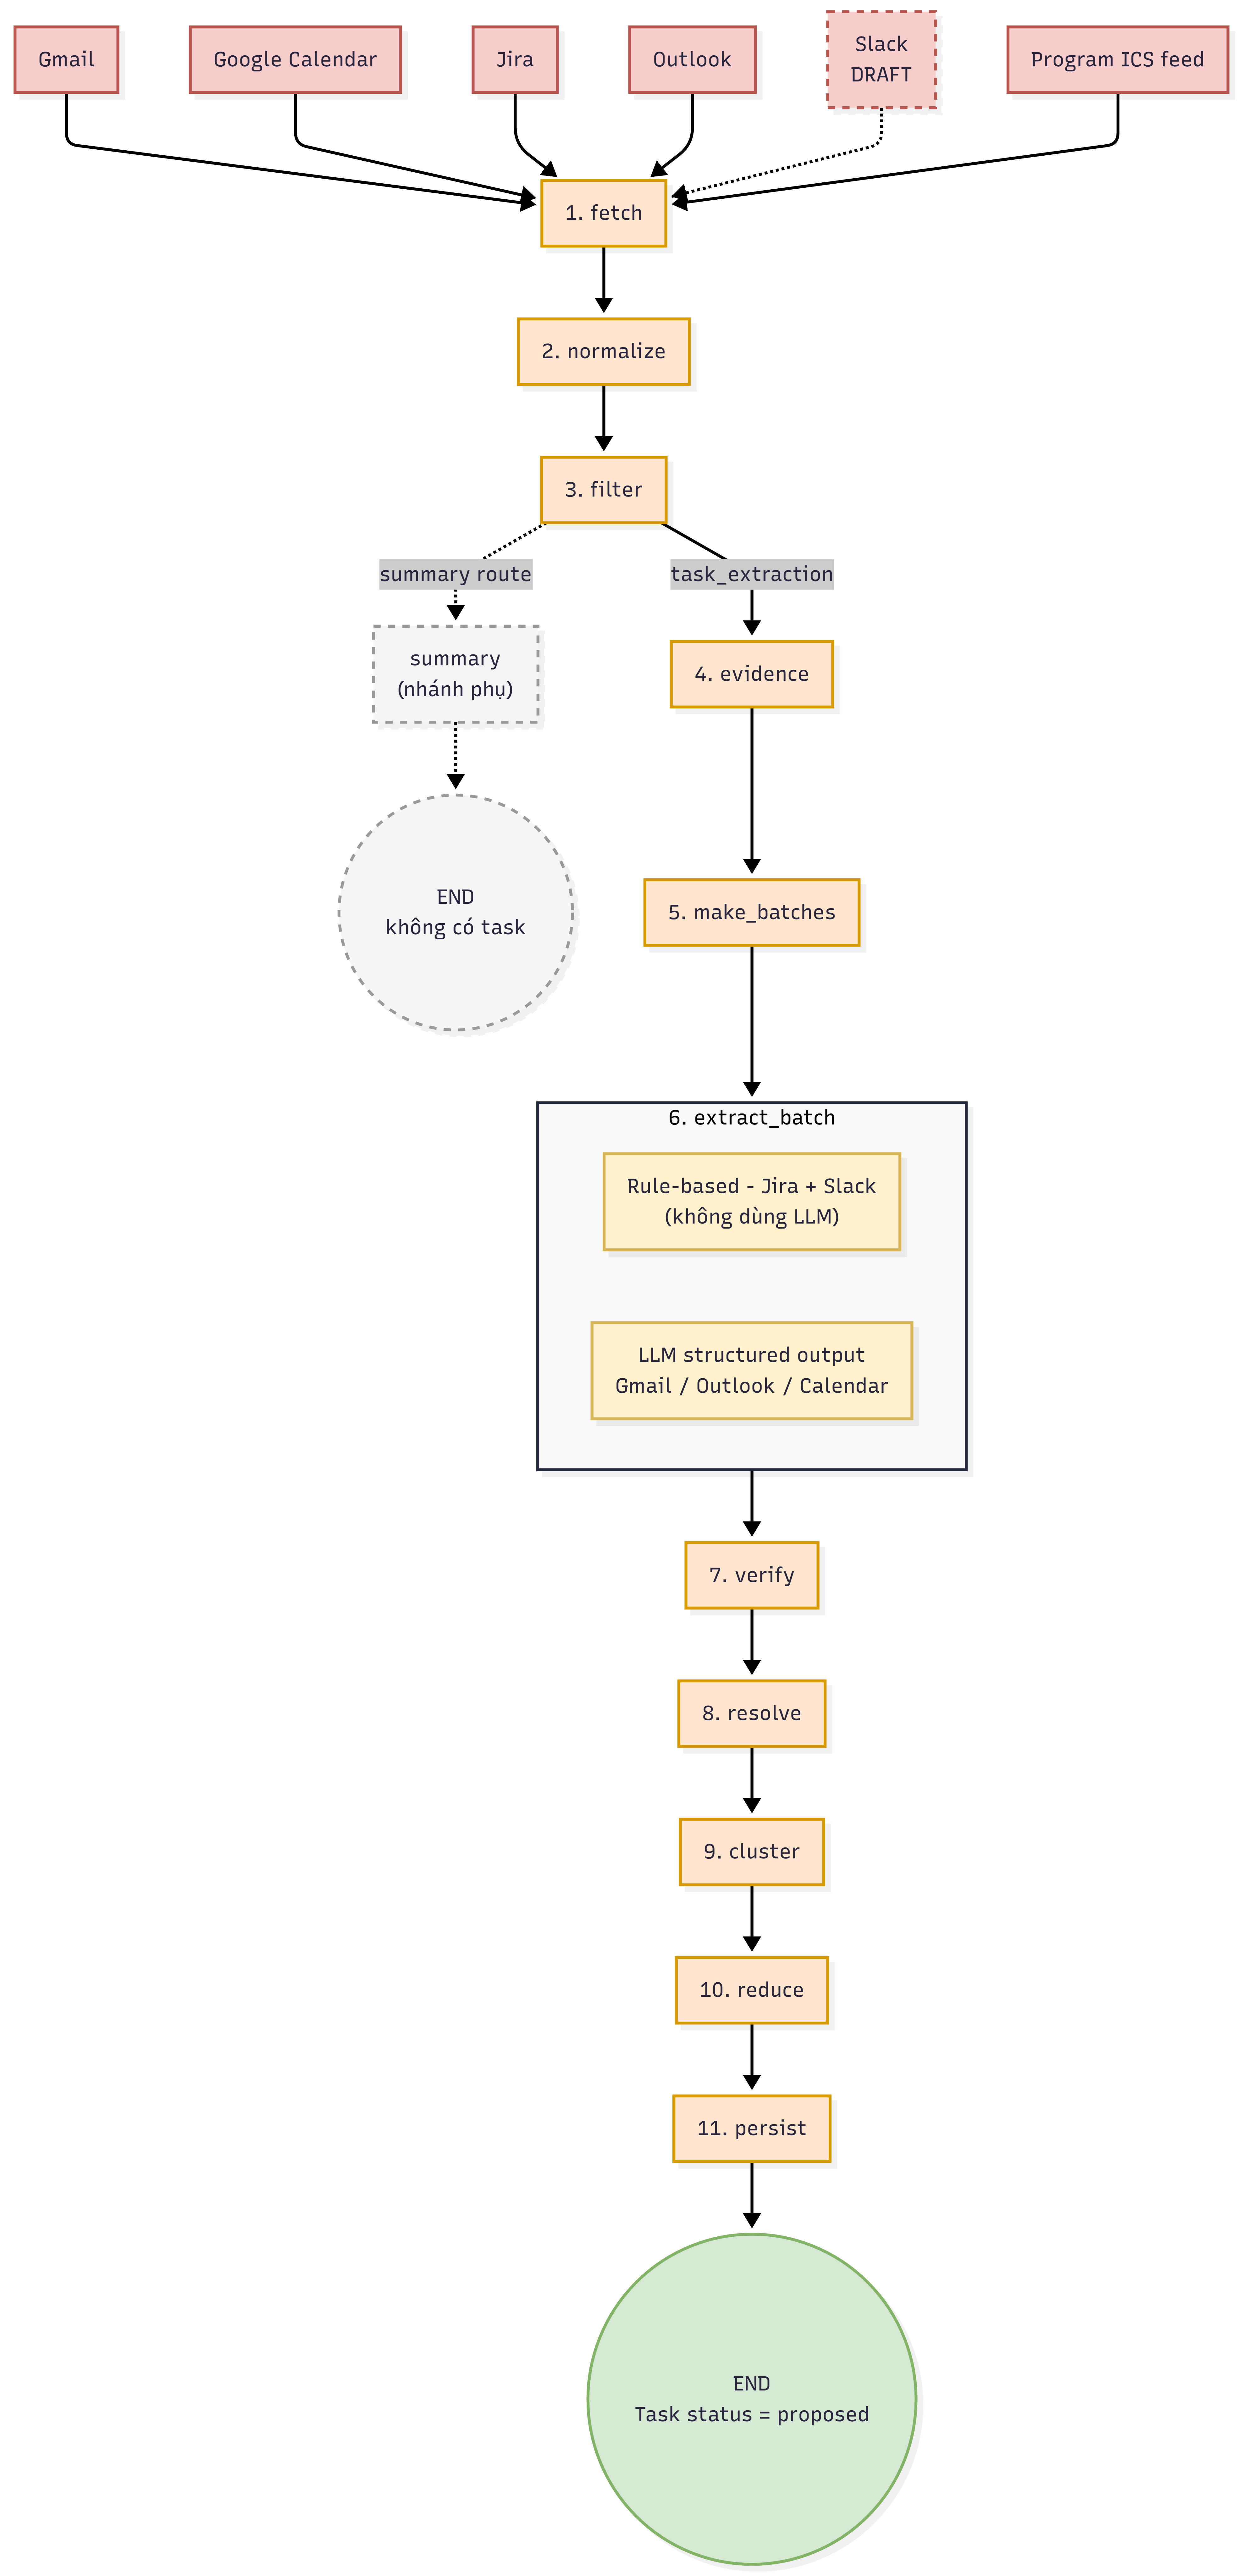
\includegraphics[width=0.98\textwidth]{components/flow.png}
\caption{Runtime/deployment flow và observability boundary từ Gate 2.}
\label{fig:sdd-deployment-flow}
\end{figure}

\subsection{Environment, rollout và rollback}
\begin{longtable}{p{3.0cm}p{4.5cm}p{6.9cm}}
\caption{Contract vận hành triển khai}\label{tab:sdd-deploy-contract}\\
\toprule Hạng mục & Thiết kế hiện tại & Quy tắc release \\ \midrule
\endfirsthead
\toprule Hạng mục & Thiết kế hiện tại & Quy tắc release \\ \midrule
\endhead
Frontend & Web build/Vercel; mobile EAS/TestFlight/native build & Web/mobile build mang version; widget chỉ pass trên native build/device evidence. \\
Backend/worker & Docker Compose trên VM, backend và worker deployable riêng & Chỉ deploy exact verified SHA; fast path recreate backend/worker, không restart shared dependency. \\
Data/runtime & PostgreSQL, Redis, object storage, production environment trên VM & Migration compatibility/rollback phải có trước deploy; production env không copy vào Git/test. \\
Health/monitoring & Health endpoint, structured log, Prometheus/Grafana/LangSmith & Verify health, error, queue, source freshness, model cost/latency sau rollout. \\
Rollback & Previous image/artifact và runbook & Ghi rollback target trước rollout; rollback không được làm mất data hoặc bypass migration safety. \\
\bottomrule
\end{longtable}

\section{Quyết định thiết kế và rủi ro mở}
\begin{longtable}{p{3.0cm}p{3.4cm}p{5.1cm}p{3.0cm}}
\caption{Decision log và open risk}\label{tab:sdd-decision-log}\\
\toprule Chủ đề & Lựa chọn hiện tại & Lý do/ràng buộc & Owner/follow-up \\ \midrule
\endfirsthead
\toprule Chủ đề & Lựa chọn hiện tại & Lý do/ràng buộc & Owner/follow-up \\ \midrule
\endhead
Architecture & Modular monolith + worker & Giảm operational overhead, giữ transaction/auth/audit gần nhau trong pilot; module boundary vẫn rõ. & Dũng quyết định split khi load/ownership evidence yêu cầu. \\
API & FastAPI REST/SSE & Hợp với web/mobile/extension, typed validation và streaming conversation. & Phong/An giữ version/error contract. \\
Data & PostgreSQL canonical + Redis coordination & Quan hệ user/source/task/audit cần consistency; Redis không là source of truth. & Dũng cập nhật ADR/diagram nếu runtime đổi. \\
AI execution & Capability-aware lane, tool binding, structured output & Capability/safety trước cost; no tool/model may alter scope or write policy. & ADR-005 còn Proposed; chỉ claim behavior có evidence. \\
Action & Draft-preview-confirm + idempotency & Chặn external write tự ý và retry duplicate. & QA kiểm no-write-before-confirm. \\
Connector scope & Connector/channel hiện diện trong code không tự thành P0 & Telegram/Slack/Outlook cần đối chiếu PRD/ADR trước release claim. & Dũng kiểm scope; Phong/An implement. \\
Retention/RPO/RTO & Chưa chốt value & Không điền số không có authority hoặc claim production-scale readiness. & Dũng tạo decision trước scale claim. \\
\bottomrule
\end{longtable}

\section{Traceability từ yêu cầu đến thiết kế và kiểm thử}
\label{sec:trace}
\begin{longtable}{p{2.5cm}p{4cm}p{4.3cm}p{3.2cm}}
\caption{Ánh xạ SRS sang implementation design và STD}\\
\toprule SRS & Component/contract & Boundary & STD evidence \\ \midrule
\endfirsthead
\toprule SRS & Component/contract & Boundary & STD evidence \\ \midrule
\endhead
FR-01/02/08/22 & Identity, consent, connection, privacy & JWT/OAuth, scope, revoke/pause/delete, AI consent. & Auth/connection/revoke/delete denial. \\
FR-03/06/12/13/15/16 & Connector, pipeline, evidence, context, briefing, audit & Bounded fetch, provenance, run outcome/coverage, memory scope. & Sync/retry/restart/idempotency/citation/redaction. \\
FR-04/05/09/10/18--21 & Task, planning, calendar, note, file intake, reminder & Draft-confirm, validation, plan/replan, conflict, idempotency, audit. & No-write-before-confirm, planning, file reject, conflict. \\
FR-07/14/17 & Retrieval, agent, tool guard, priority & Scoped evidence, citation/abstain, tool capability, rationale. & Citation, unanswerable, priority, tool/schema/injection. \\
FR-11/23/24/NFR-05 & Web/mobile/extension/admin/channel & API-only auth, accessible state, native widget, role/delivery boundary. & UI/native/role/channel smoke. \\
NFR-01--11 & Security, reliability, observability, deploy & Redaction, retry/fallback, health/rollback, quality protocol. & Privacy, chaos, latency/cost, dataset and coverage evidence. \\
\bottomrule
\end{longtable}

\end{document}
